% (c) 2020 Stefan Antonowicz
% Based off of tex found at https://github.com/ludus-leonis/nipajin
% This file is released under Creative Commons
% Attribution-NonCommercial-ShareAlike 4.0 International License.
% Please do not apply other licenses one-way.

\renewcommand{\yggResearch}{%
  \mychapter{Research}{research}
    \begin{center}
    
\includegraphics[width=\linewidth,keepaspectratio=true]{research/ResearchHeader}
    \end{center}
    \newpage
}

\renewcommand{\yggResearchText}{%

\end{multicols*}

\mybold{Research} is a catch-all term for the experimentation, analysis, reading, and application of "science" during Downtime.  Your abilities as a researcher are measured by \mybold{\myanchor{Research Pips}{research-pips}} obtained through the Philosophic virtues of Chymist and Scribe, and through \mypg{Advancement}{advancement}.  See \mypg{Philosophers}{trope-philosopher} for more information.


    Research Pips can be spent during the \mybold{Production Step} of \mypg{Downtime}{downtime}. Any Research Pips you don't spend during the Production Step are lost at the end of the step.

Research also requires an expenditure of coin, representing the bribing of librarians, rental of laboratory equipment, purchase of legal and illegal inks, payment to grave-robbers for corpses, etc. The total cost to perform Research depends on the total number of Research Pips you spend: the first 5 pips will cost you 100 \FE \myital{each}; the next 5 pips cost you 100 \AG each; and every pip after that will cost you 100 \AU For example, if you spend 12 Research pips, the total will be 500 \FE plus 500 \AG plus 200 \AU 



    \myctrtable{Y Y} {
        \thead{\# Pips} & \thead{Coin per Pip} \\
    } {
        1-5 & 100\FE \\
        6-10 & 100\AG \\
        11+ & 100\AU
    }


The Arbiter is encouraged to expand the use of Research Pips to include any kind of investigation the Adventurers might attempt during Downtime (for instance, a player may wish to research a cure to a virulent disease, or the location of the Sepulcher of the Blood God, lost for some 1,000 years). Simply set a secret difficulty in number of pips (50 for the Sepulcher, say - or 20 for the cure to the disease). The Adventurers may spend their Research Pips against this total over multiple Sessions, each time coming closer to the answer. When they spend the 50th, 20th, etc. pip, they finally find what they've been looking for. A Library in a Settlement is required to perform this type of research, and the cost for pips is the same as above.

\myfpimage{research/CowSkull}


\example{
    Craps Bastogne is a level 3 Philosopher who has dedicated his life to research - he has 6 Research Pips, and the Virtues Chymist and Scribe. He has 20\AU (or 200\AG) in his purse. Craps first scribes a spell from a Fetish he found into his Grimoire (1 Research Pip), and scribes a different spell to a new Fetish, the skin of a blind toad (1 Research Pip). He uses the toad's bile to create a Noxious Toxin (2 Research Pips), and decides to put the final 2 Pips into deciphering the map to the Somatocyst of the Slumbering Medusa (originally requiring 10 Research Pips, Craps has slowly made progress - the Arbiter notes he only has 1 pip to go, so she'd better get cracking on that dungeon!). In total he has spent 6 Research Pips for all his activities, and must pay 500 \FE \PLUS 100 \AG in total (this is the same as 150 \AG, or 15 \AU). He subtracts 15\AU from his coins, and adds the Fetish and Toxin to his inventory.  If he had been short on money, he could have instead simply spent 1 Pip on the deciphering of the map, which would have dropped his costs to 500 \FE (or only 50\AG).

}


\newpage

\begin{multicols*}{2}

  \newpage
  %%%%%%%%%%%%%%%%%%%%%%%%%%%%%%%%%%%%%%%%%%%%
%%% CHYMISTRY
%%%%%%%%%%%%%%%%%%%%%%%%%%%%%%%%%%%%%%%%%%%%
\mysection{Chymistry}{research-chymistry}

\flavor {
    You've had your say, Potion Seller but I'll have mine. You're a rascal, you're a rascal with no respect for knights. No respect for anything... except your potions!

    \myskip

    Why respect knights... when my potions can do anything that you can?
  }


\callout {
    \mytable{Y Y} {
        \thead{\# Pips} & \thead{Coin per Pip} \\
    } {
        1-5 & 100\FE \\
        6-10 & 100\AG \\
        11+ & 100\AU
    }
}

Through the careful study of the structure and properties of certain natural substances, the Researcher is able to refine, transform and energize their quintessence to produce new and powerful essences:


\callout {\footnotesize{
\mybullet {
  \item \mylink{Elixirs:}{research-chymistry-elixirs} various tonics, powders, sera, and unguents.
  \item \mylink{Laudanum:}{research-chymistry-laudanum} opiatic preparations for treating \mylink{Madness!}{injury-insanity-madness}.
  \item \mylink{Malignants:}{research-chymistry-malignants} poisons, toxins, and acids.
  \item \mylink{Grenades:}{research-chymistry-grenades} petards, trombes, and bombs.
}}}

\begin{center}
  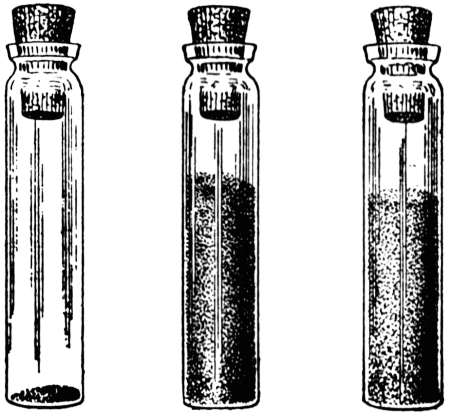
\includegraphics[scale=.35]{research/Chymistry}
\end{center}


\cbreak

\mysubsection{Elixirs}{research-chymistry-elixirs}

Elixirs can be encountered in four different forms:

\mybold{Tonics}  are mixtures of booze, narcotics, and other things you probably don't want to know about. They must be drunk.

\mybold{Powders} can be drunk (in wine), inhaled, or smoked.  If you blow a powder in some Monster’s face, the Monster has to be able to breathe (so they don't work on undead, for example).

\mybold{Sera} need to be injected via a \mylink{Syringe}{gear-equipment}.  If the recipient is a person, they have to have a vein of some kind.  If the recipient is an object, it has to be something a needle could pierce (like an apple).

\mybold{Unguents} include oils, salves, lubricants, and pastes - basically anything you rub on things (heh heh).  They're usually super viscous and anyone will know the moment they try to drink it.  You can coat a weapon with an unguent  and "apply" it to a Monster by injuring them with the weapon (1 point of damage or more to Flesh).  If your attack misses the unguent doesn't rub off, but if you hit armor / scales / etc. without piercing Flesh, it does.  Unguents can be rubbed on someone who is who is unconscious or petrified.  The can’t be eaten as they taste shitty and will most likely be spit out, unless the eater is extremely ravenous or extremely stupid.


When created, an Elixir has \UDD{d4}. The following are the most common Elixirs:

\newpage 

\CHYMISTRY[
    Name=Al-Farabi's Calming Injection,
    Link=chymistry-al-farabis-calming-injection,
    Type=Sera,
    Pips=5,
    Time=Weeks
]

  The injected creature ceases immediately to be \mylink{Enraged}{effect-enraged}, \mylink{Shaken}{effect-shaken}, \mylink{Frenzied}{monster-trait-frenzied}, or \mylink{Disgusted}{effect-disgusted}.  If the creature is \mylink{Zoological}{monster-trait-zoological}, they become passive and docile.  Creatures under the effect of the Calming Injection cannot attack unless they are attacked first (if they are attacked, the effects of the injection immediately end). Unwilling creatures get a Save to negate; the effect of passivity lasts until the end of the Session.

  \CHYMISTRY[
    Name=Boyle's Sharpening Paste,
    Link=chymistry-boyles-sharpening-paste,
    Type=Unguent,
    Pips=2+,
    Time=Days
  ]

  When rubbed on the blade of a Stabbing or Chopping weapon, the weapon deals extra damage then next time it is used. The oil rubs off after a successful strike. The amount of damage depends on the number of Research Pips used:  (2) +d6; (5) +d10; (10) +d16.  


  \CHYMISTRY[
    Name=Brahe's Efficacious Sealant,
    Link=chymistry-brahes-efficacious-sealant,
    Type=Unguent,
    Pips=5,
    Time=Weeks
  ]


  A fast-drying paste that is capable of bonding stone, glass, wood, or metal (but not flesh). The Sealant lasts forever, and each use can cover an area roughly 10cm square.


\CHYMISTRY[
    Name=Chyme's Nerve Tonic,
    Link=chymistry-chymes-nerve-tonic,
    Type=Tonic,
    Pips=2+,
    Time=Days
]

This tonic grants the imbiber a +1 to all \RO and \RB tries until they take a \mylink{Bivouac}{combat-resting-bivouac}; for each additional 2 Research Pips you spend, you can increase the potency by +1 (up to +4 to all tries).  The imbiber cannot take a \mylink{Breather}{combat-resting-breather}, however - they are far too restless.

  \CHYMISTRY[
    Name=Cold and Drowsy Humor,
    Link=chymistry-cold-drowsy-humor,
    Type=Powder,
    Pips=5,
    Time=Days
  ]

  The imbiber stops breathing for the remainder of the Session.  They can feign death or travel underwater, are not affected by inhaled powders or gases, and are unable to speak - meaning they cannot perform certain Arcana or Vulgates.  Unwilling victims get a \SAVE{Toxins}.

\CHYMISTRY[
  Name=Cuckold's Courage,
  Link=chymistry-cuckold-courage,
  Type=Tonic,
  Pips=2,
  Time=Days
]

When quaffed, Cuckold's Courage restores 4 Grit (even over your \MAX). For every sip, the imbiber must try to \RSTRY{\VIG}; Failure gives the drinker a level of \mylink{Drunk}{effect-drunk}. If you fail your \RSTRY{\VIG} when you are at \mybold{Drunk -4}, you \mylink{Overdose}{gear-narcotics-overdose}.


  \CHYMISTRY[
    Name=Dastin's Basic Talc,
    Link=chymistry-dastins-basic-talc,
    Type=Powder,
    Pips=5,
    Time=Days
  ]


  Immediately neutralizes any acid it comes in contact with. 


  \CHYMISTRY[
    Name=Faivre's Aqua Grease,
    Link=chymistry-faivres-aqua-grease,
    Type=Unguent,
    Pips=2,
    Time=Days
  ]

  A pale grease that can be rubbed on equipment to completely protect it against damage from water exposure. If rubbed on the body, allows you to swim without tiring for Hours.


\CHYMISTRY[
  Name=Fulcanelli's Clarifying Elixir,
  Link=chymistry-fulcanelli-clarifying-elixir,
  Type=Tonic,
  Pips=5,
  Time=Weeks
]

This tonic grants the drinker a bonus to resist any effects from the \mylink{Secrets of the Mind}{arcana-wizardry-secrets-alignment}. If the imbiber wouldn't normally get a Save vs. the effect, they now do; if they \mybold{do} get a Save, they can now make their try at +4.  If imbibed when the drinker is already under some effect of the Mind, the drinker immediately gives the imbiber a new Save.  This tonic immediately breaks the effects of the \mylink{Philter of von Fuchs}{chymistry-philter-von-fuchs}.




  \CHYMISTRY[
    Name=Grimm's Stuporous Preparation,
    Link=chymistry-grimms-stuporous-preparation,
    Type=Sera,
    Pips=5,
    Time=Weeks
  ]

  An injected creature immediately falls into a slumber in all ways like \mylink{Sleep}{secrets-sleep} (can't be awakened except by a slap, doesn't effect a creature of greater than 4 \HD) unless they Save vs. Toxins.

 If this Sera is injected into a piece of \mylink{Forbidden Fruit}{marvels-forbidden-fruit} and the fruit is ingested, the effect of the Sleep acts as a \mylink{Greater Curse}{table-greater-curses} unless a \SAVE{Toxins} try is made. The sleep is permanent until the curse is fed to a \mylink{Hekaphage}{occultism-hekaphage} or until the creator of the \mylink{Forbidden Fruit}{marvels-forbidden-fruit} either lifts the curse, or is slain. While asleep the creature is in a state of suspended animation - they do not age, and do not need to eat or drink - but they can still be killed in the normal means (dagger through the heart, etc). Putting a creature into suspended animation will stop the effects of progressing disease and toxins.


\CHYMISTRY[
  Name=Liebnitz Purgation,
  Link=chymistry-liebnitz-purgation,
  Type=Tonic,
  Pips=5,
  Time=Days
]


If imbibed while under the effects of an ingested \mylink{Toxin}{malignants-toxins}, the poison is immediately vomited up and ceases to affect the victim.


\CHYMISTRY[
  Name=Philter of von Fuchs,
  Link=chymistry-philter-von-fuchs,
  Type=Tonic,
  Pips=2+,
  Time=Weeks
]

When imbibed, the drinker will fall under the sway of whoever gave them the tonic (treat as if someone spoke a \mylink{Charm}{secrets-charm} Secret). Save vs. Toxins negates the effect, but if the victim should fail the duration depends on the number of Research Pips used:  (2) Days; (5) Weeks; (10) Months. Won't affect creatures who are immune to the \mylink{Secrets of the Mind}{arcana-wizardry-secrets-alignment}.


  \CHYMISTRY[
    Name=Powdered Bezoar,
    Link=chymistry-powdered-bezoar,
    Type=Powder,
    Pips=2+,
    Time=Days
  ]


  When sprinkled on food or into a beverage, the Powdered Bezoar has a chance to neutralize the Toxin contained inside. The chance of success depends on the number of Research Pips spent: (2 Pips) 3-in-6; (4 Pips) 5-in-6; (6 Pips) Automatic Success. If a roll is needed, it is made in secret by the Arbiter.



  \CHYMISTRY[
    Name=Tesla's Silver Wash,
    Link=chymistry-teslas-silver-wash,
    Type=Unguent,
    Pips=5,
    Time=Weeks
  ]

  When applied to a 1-handed weapon, the weapon becomes permanently imbued with silver. Requires an \mylink{Ingot of silver}{settlements-money}.


  \CHYMISTRY[
    Name=Wallace's Anesthetic,
    Link=chymistry-davys-soothing-anesthetic,
    Type=Sera,
    Pips=5,
    Time=Days
  ]

  The injected creature feels any pain as pleasure until the end of the Session. Often surreptitiously given to those undergoing torture, or going under the knife for surgery. 

If the imbiber is an Adventurer, the Arbiter will roll damage against you in secret, and keep track of your Grit and Flesh for you (you keep track of your Armor). You can't ask the Arbiter how many Grit or Flesh you have left, but you can ask them how you look ("you're pretty beat up", "you're missing an arm", etc.).

If the imbiber is a Monster, treat as if the Monster had \mylink{Fanatical}{monster-morale} morale. Attacks against the Monster do +2 damage.


  \CHYMISTRY[
    Name=Wei Boyang's Alkahest,
    Link=chymistry-wei-boyangs-alkahest,
    Type=Unguent,
    Pips=5,
    Time=Weeks
  ]

  This oil will dissolve any adhesive (including \mylink{Brahe's Efficacious Sealant}{chymistry-brahes-efficacious-sealant}).  Each use can cover an area roughly 10cm square.


  \CHYMISTRY[
    Name=Wordwarp,
    Link=chymistry-wordwarp,
    Type=Sera,
    Pips=5,
    Time=Weeks
  ]

  Any creature injected with this serum is affected with severe dyslexia should the fail a Save vs. Toxins. They are unable to read or write (including from Grimoires or Fetishes) for the rest of the Session.


  \CHYMISTRY[
    Name=Woundseal,
    Link=chymistry-woundseal,
    Type=Powder,
    Pips=2,
    Time=Days
  ]


  Sprinkling this powder on a wound immediately stops all effects of \mylink{Bleeding}{effect-bleeding}.

  \myimage{research/Chymistry_2}


\mysubsection{Laudanum}{research-chymistry-laudanum}

\flavor{We're all mad here. \\~ \Tilde The Cheshire cat, "Alice's Adventures in Wonderland"}

You may use your special concoctions to remove \mylink{Madness!}{injury-insanity-madness} from an unfortunate victim. Each Madness! removed requires 1 Research Pip (and 100\AG). For every Madness! removed by a \mylink{Chirurgeon}{gear-services}, multiply the costs by 5x (500\AG).



\mysubsection{Malignants}{research-chymistry-malignants}


\mybigbold{\myanchor{Acids}{malignants-acids}}

Acids can be created as liquids or powders, stored in special containers that don't react with their volatile nature (the relative fragility of these containers is at the Arbiter's discretion). Acids will dissolve flesh, stone, wood, or iron and are often used for etching, ruining locks, and pouring on people you hate.  \mybold{Each of the following effects requires 2 Research Pips}:


  \mynumlist {
    \item If the acid hits Flesh, the victim takes d4 damage for d4 Moments. If it hits Armor, the Armor \UD must be rolled at the top of every Moment.
    \item The acid can melt an area 100cm cubed of wood, metal, or stone in Minutes.
    \item When thrown on the ground, the acid will create an acrid plume of smoke that causes coughing and choking for Minutes to everything Nearby (-2 to \RO and \RB attempts).
  }

  You can sunder your Shield to negate the effect of acids thrown on you. Acids take \mybold{Days} to make.


\mybigbold{\myanchor{Toxins}{malignants-toxins}}

\flavor{Such mortal drugs I have, but Mantua’s law / Is death to any he that utters them. \\~ \Tilde The Apothecary, "Romeo and Juliet"}

Venoms, blights, poisons, blights, and banes are grouped under \mybold{Toxins}. Like \mylink{Elixirs}{research-chymistry-elixirs}, Toxins may be created as Tonics, Unguents, Sera, or Powders. The efficacy of the poison depends on the number of Research Pips invested:

  \mytable{Y Y Y Y} {
    \thead{Type} & \thead{\faClock[regular]} & \thead{Pips} & \thead{Downtime} \\
  } {
     Noxious & d6 & 2  & Days \\
     Deadly & d10 & 5 & Weeks \\
     Lethal & d16 & 10 & Months \\
  }

  When you are first afflicted by a Toxin, try a \SAVE{Toxins}; if you succeed, nothing happens.

  If you fail, the Arbiter should start a timer. Immediately roll the Toxin's \Duration and apply its result as damage. Every real-world minute afterwards, roll the \Duration for the Toxin and apply its result as damage. Any damage from Toxins is dealt to Grit first (wearing away your will to live) followed by Flesh. You cannot heal Grit while under the effects of a Toxin.  Note that when a Failure is finally rolled, the 1 or 2 points of damage is still dealt to your Adventurer.

 Again, note that this is a \mybold{Duration} die, meaning the effect of the poison ends if you roll a 1 or a 2, and any other roll moves the die \DCDOWN.


\cbreak

  \example {
Andre Preneur (Grit 4, Flesh 6) drinks a Deadly (d10) Powder dissolved in a glass of wine. Andre tries \SAVE{Toxins} - and fails, so the Arbiter starts a timer and Andre rolls a d10 and gets a 4. Andre applies 4 damage and is now at 0 Grit and 6 Flesh. His Band starts shouting excitedly over one another trying to figure out what to do. After a minute of indecision, the die moves \DCDOWN (d8) and Andre rolls again - getting a 6. Oof! Andre is now \mylink{Dying}{combat-dying}.  He will now need to make a \DEATH try every time he takes damage. The Band holds its breath as the timer marks the end of the 3rd minute ...
  }

  \myimage{research/Poison}


\newpage



\mysubsection{Grenades}{research-chymistry-grenades}

\flavor {
    Anytime I had a problem and I threw a Molotov cocktail, boom! Right away, I had a different problem. 

    ~\Tilde Jason Mendoza, The Good Place
}

Grenades are Thrown \INT weapons that have the \mylink{Splattering Attribute}{weapon-attribute-splattering}. They have different effects and strengths depending on the number of Research Pips spent. Each Grenade is a significant item and has a \mylink{Burden}{gear-burden} of 1 (as they must be handled \myital{carefully}!). They take \mybold{Weeks} to make (but you can make as many as your Research Pips will allow).


\mybold{Each Grenade can only have 1 effect:}


  \mytable{Y Y} {
    \thead{Type} & \thead{Pips} \\
  } {
     Acid & 2 \\
     Bomb & 3 \\
     Chaos & 4 \\
     Concussive & 2 \\
     Explosive & 2 \\
     Fire & 2 \\     
     Flashbang  & 1  \\
     Frag & 1 \\
     Illuminating & 1  \\
     Poison Gas & 3 \\
     Screaming & 3 \\
     Smoke & 1  \\
  }

  \myhighlight{Acid}{grenade-acid}

  You may place an \mylink{Acid}{malignants-acids} you have created inside of the Grenade to be thrown.

  \myhighlight{Bomb}{grenade-bomb}

  Creatures Close to the point of explosion take d10 damage (\SAVE{Toxins} for half).  The bomb can have a fuse.

  \myhighlight{Chaos}{grenade-chaos}

   Creatures Close to the point of explosion must \SAVE{Toxins} or become \mylink{Befuddled}{effect-befuddled} and \mylink{Enraged}{effect-enraged} (the source of their rage is a random Close target) for \DUR{d4}.




\cbreak

\myimage{research/Molotov}

  \myhighlight{Concussive}{grenade-concussive}

   Creatures Close to the point of explosion must \SAVE{Toxins} or be \mylink{Knocked Out}{effect-knocked-out} for \DUR{d4}.
 
  \myhighlight{Explosive}{grenade-explosive}

  Creatures Close to the point of explosion take d8 damage (\SAVE{Toxins} for half).


  \myhighlight{Fire}{grenade-fire}

   Creatures Close to the point of explosion must \SAVE{Toxins} or become \mylink{Enflamed}{effect-enflamed}. Flammable things also catch fire (including oil).

  \myhighlight{Flashbang}{grenade-flashbang}

   Creatures Close to the point of explosion must \SAVE{Toxins} or be \mylink{Stunned}{effect-stunned} for \DUR{d4}.

  \myhighlight{Frag}{grenade-frag}

  Creatures Close to the point of explosion take d6 damage (\SAVE{Toxins} for half).

\end{multicols*}
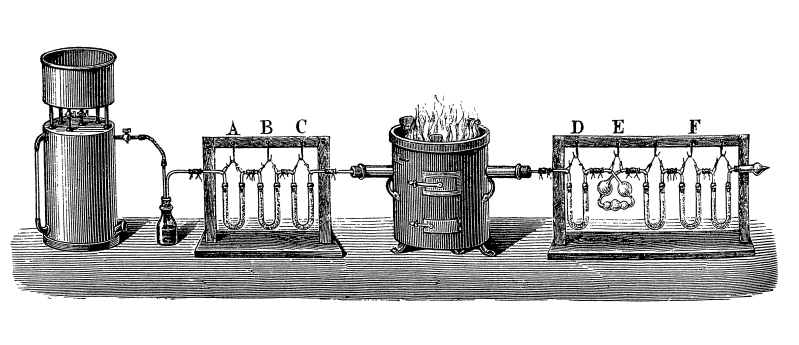
\includegraphics[width=\linewidth]{research/Lab}
\begin{multicols*}{2}

  \myhighlight{Illuminating}{grenade-illuminating}

  Creatures Close to the point of explosion must \SAVE{Toxins} or be \mylink{Blinded}{effect-blinded} for \DUR{d4}.

  \myhighlight{Poison Gas}{grenade-poison}

  You may place a \mylink{Toxin}{malignants-toxins} inside of the Grenade to be thrown.

  \myhighlight{Screaming}{grenade-screaming}

   Creatures Close to the point of explosion must \SAVE{Toxins} or become \mylink{Afraid}{effect-afraid} for \DUR{d4}.

\cbreak
   
  \myhighlight{Smoke}{grenade-smoke}

   Everything Close to the area of impact is enveloped in smoke. The smoke acts as if a Philosopher had spoken the Secret of \mylink{Fogbank}{secrets-fogbank}, though the smoke won't move from the spot of impact. The smoke lasts for \DUR{d4}.

\newpage

  \newpage
  %%%%%%%%%%%%%%%%%%%%%%%%%%%%%%%%%%%%%%%%%%%%
%%% INSCRIPTION
%%%%%%%%%%%%%%%%%%%%%%%%%%%%%%%%%%%%%%%%%%%%



\mysection{Inscription}{research-inscription}


\callout {
    \mybold{Research Costs}

    \mytable{Y Y} {
        \thead{\# Pips} & \thead{Coin per Pip} \\
    } {
        1-5 & 100\FE \\
        6-10 & 100\AG \\
        11+ & 100\AU
    }
}


Incantations, symbols, and engravings; arcane calligraphy, runed manuscripts, symbols etched on papyri and clay tablets. Through Inscription, the skilled Philosopher captures a small part of the Void and binds it inside a written word. Practicing Inscription requires the Settlement where you're taking Downtime to have a \mypg{Library}{gear-services}. Inscription only requires \mybold{Days} of Downtime, and covers:

\mybullet{
  \item \mybold{Transcription:} Writing \mypg{Secrets}{arcana-wizardry-secrets} from and to \mybold{Grimoires and Fetishes} (see below).
  \item \mybold{Tattooing:} Branding and marking the flesh of living things with magical symbols.
  \item \mybold{Sigils:} Etching and inscribing magical runes.
}

  \myimage{research/Inscription_1}

\mysubsection{Transcription}{research-inscription-transcription}

Transcription is used to copy Secrets from a Fetish into a Grimoire, or from a Grimoire onto a Fetish. You cannot inscribe Secrets from your own \mypg{skull}{arcana-wizardry-skull} onto a Grimoire or Fetish (your brain is in the way).

Additionally, you may attempt to carefully translate the Grimoires of other Sorcerers - but be careful! A mistake can lead to serious unpleasantness (see \mybold{Grimoire Traps} below).



\myhighlight{Translation}{inscription-translation}

A Grimoire must be carefully cataloged, keyed, and decrypted in order to be read by another. Each Research Pip you spend increases the die you may roll in order to successfully translate a Grimoire. If you roll a Failure, you must roll on the Grimoire Traps table - otherwise, you may successfully copy the contents of the foreign Grimoire onto a Fetish or into your own Grimoire. \mybold{You must translate the foreign Grimoire every time you wish to read it}, but when you do you may inscribe as many Secrets as you're able.

    \mytable{Y Y} {
        \thead{\# Pips} & \thead{Die} \\
    } {
        1 & d3 \\
        2 & d6 \\
        3 & d10 \\
        4 & d16 \\
        5 & d24 \\
        6 & \myital{Automatic Success} \\
    }

\myhighlight{Inscribing}{inscription-inscribing}

Each Secret you wish to Inscribe costs 1 Research Pip.

You can write a Secret from a Fetish, \mypg{Sorcerer's Skull}{arcana-wizardry-skull}, or untrapped foreign Grimoire (see above) to your Grimoire.  You can also write a Secret from your Grimoire to a Fetish. See the section on \mybold{Fetishes} below for more info.

You cannot copy a Fetish to another Fetish, and you cannot copy Secrets from \myital{your} skull to a Grimoire or Fetish (your brain is in the way).


\mysubsection{Tattooing}{research-inscription-tattoo}

Only the most skilled scriveners dare to etch the Void into the flesh of the willing. \mybold{Each Tattoo you wish to create costs 6 Research Pips}.  The most common Tattoos are below - invent more with the Arbiter!


\myhighlight{Dagger (Limb)}{sorcerer-tattoo-dagger}

Touching the dagger immediately brings it into your hand.  Place the dagger back on the limb returns it to being a tattoo.  The dagger is a normal iron dagger when it is separated from your body.

\myhighlight{Torch (Limb)}{sorcerer-tattoo-torch}

As dagger above.  The torch never goes out.

\myimage{research/Tattoo}

\cbreak

\myhighlight{Compass (Limb)}{sorcerer-tattoo-compass}

Always points towards true north.  

\myhighlight{Quill and Scroll (Back)}{sorcerer-tattoo-quill-scroll}

The quill can be removed as the Dagger, above - and given to someone else.  Anything that the other person writes with the quill will appear on the scroll tattooed on your flesh ... painfully.  The writing disappears in Minutes.

\myhighlight{Eye (Palm)}{sorcerer-tattoo-eye}

The tattooed can see through the eye as if it were one of their normal eyes.

\myhighlight{Rope (Neck, Arms, Legs, Torso}{sorcerer-tattoo-rope}

As Dagger above, but uncoils from the body into 25m of rope. Needs to be completely rewound around the person to return to being a tattoo.


\myhighlight{Mermaid (chest or neck)}{sorcerer-tattoo-mermaid}

In addition to the tattoo, the Researcher inscribes a \mybold{Wizard Sigil} (see below) on a different non-living object (traditionally a ship in an open bottle or a scrimshawed whale bone). When the tattooed creature draws breath, they inhale the air immediately around the object marked with the Sigil, instead of the air (or lack thereof) surrounding themselves. This means that as long as the object isn't immersed in water, surrounded by poison gas, locked in an airtight container, etc. the tattooed creature can breathe as normal (even if under water, surrounded by poison gas, locked in an airtight container, etc.) Erasing the Wizard Sigil permanently breaks the connection between the tattoo and the object.

\newpage

\mysubsection{Sigils}{research-inscription-sigils}

Hieroglyphs, runes, seals, and marks - Sigils are magical writing inscribed onto the surfaces of objects. Sigils are very obvious - they glow slightly and exude an indefinable arcane mystery - but what a Sigil actually \myital{does} can only be guessed at (or with a successfully \mybold{Skill: Lore} try). 

Some Sigils remain even after their magic is exhausted, meaning a Sigil you encounter may be "lifeless". Only the Researcher who created a Sigil or someone skilled in the \mypg{Whispers of Sun Wukong}{vulgate-whisper-sun-wukong} can \mybold{Erase} a Sigil once it's been inscribed. For a Researcher to Erase a Sigil, they need only place their finger on it and read its name aloud (note: the finger does not need to be attached to the hand, and the finger doesn't have to have flesh on it).  Only the Researcher who etched the Sigil knows its "true name", but you may be able to divine it through research in a Library, creative use of \mypg{Descrying}{occultism-descry}, torture, etc.

\mybold{Unless otherwise specified, a Sigil can only be placed on something that is generally immobile and not alive} - a door, a wall, the floor, a statue, etc.  The author is immune to any Sigils inscribed by themselves, where appropriate. Finally, in cases where Sigils may "activate" more than once before they become lifeless, they require Minutes to recharge themselves.

\myimage{research/Sigil1}

\cbreak


\myhighlight{Novice Sigils}{sigils-novice}

\callout{
    \begin{center}
    Novice Sigils cost 2 Research Pips
    \end{center}
}


\myanchor{\mybold{Chaining Sigil}}{inscription-sigil-chaining}  

A Chaining Sigil can be inscribed and "married" to another Sigil.  The Chaining Sigil must be created at the same time as its partner Sigil.  If a Chaining Sigil is Erased, the Sigil it is partnered with will immediately manifest.


\myanchor{\mybold{Talking Sigil}}{inscription-sigil-talking} 

When anyone comes Close to an object with a Talking Sigil on it, it will yell out a word at ear-splitting volume.  It will repeat this word for 1 real-world minute before becoming lifeless.  Each additional word or minute you want the Talking Sigil to speak, you must spend an additional 1 Research Pip.

\myanchor{\mybold{Warding Sigil}}{inscription-sigil-warding}

This glyph can only be placed on something that is closed: a book, a lock, a chest but not a sword in a scabbard or someone's mouth (Arbiter's discretion).  If the warded item is opened, the Sigil immediately becomes lifeless.

When anyone comes Close to an item with a Warding Sigil on it, they must \SAVE{Hexes} or find themselves compelled to ignore the object - put the book down, leave the lock where it is, walk away from the door, etc. The Warding Sigil has no effect on beings who are immune to the \mypg{Secrets of the Mind}{arcana-wizardry-secrets-alignment}. For each additional Research Pip you spend, the Warding Sigil inflicts a -1 penalty to the Save (maximum -4).

\myanchor{\mybold{Wizard Sigil}}{inscription-sigil-wizard}

The most basic Sigil, necessary to prepare a weapon, object, or person as a receptacle for magic. Each Wizard Sigil is as unique as a fingerprint; if you're familiar with the work of a certain Philosopher, you'll notice their Wizard Sigil right away.  Otherwise, you can identify the owner of a Sigil with a successful \mybold{Skill: Lore} try at the Arbiter's discretion.

For an additional Research Pip, a Wizard Sigil can be made temporarily "portable". The Sigil will appear inscribed upon the palm of your hand until the end of the Session. By touching your hand to an object, you can transfer the Sigil to it, where it will become permanent and remain until Erased. If you don't transfer the Wizard Sigil by the end of the Session, it disappears.


\myhighlight{Warlock Sigils}{sigils-warlock}

\callout{
    \begin{center}
    Warlock Sigils cost 7 Research Pips
    \end{center}
}


\myanchor{\mybold{Cursing Sigil}}{inscription-sigil-cursing}

Working with someone versed in the arts of \mypg{Cunning}{cunning}, you may place a \mypg{Malison}{occultism-malison} into a Cursing Sigil. After you inscribe the Sigil, the occultist can place a \mypg{Lesser or Greater Curse}{cunning-curses} inside of it. 

When anyone comes Close to an object with the Sigil on it, they must \SAVE{Hexes} or fall victim to the curse. If there is more than 1 target, they must all Save.  The Sigil becomes lifeless after it delivers its curse.  For each additional Research Pip you spend, the Cursing Sigil inflicts a -1 penalty to the Save (maximum -4).


\myanchor{\mybold{Elemental Sigil}}{inscription-sigil-elemental}

When inscribing this Sigil, choose an elemental type (lightning, fire, wind, etc.) Any creature who comes Close to an Elemental Sigil triggers its effect, blasting the entire Close area with its elemental payload. The Sigil deals twice the number of Research Pips spent in damage (Save for half), and becomes lifeless after it explodes.

\myanchor{\mybold{Petrifying Sigil}}{inscription-sigil-petrifying}

All creatures who comes Close to the Petrifying Sigil must Save or gain a permanent \effect{Paralyzed}. The effect lasts until the Sigil is Erased. You are aware of everything going on around you, but you do not age when you are in this state (most Mortals who are "rescued" from a Petrifying Sigil centuries after their mishap are hopelessly insane). The Sigil will affect a number of creatures equal to the number of Research Pips spent before becoming lifeless.

\myanchor{\mybold{Portal Sigil}}{inscription-sigil-portal}

Portal Sigils must be placed on doors, gates, or entrances (Arbiter's discretion). The Portal Sigil is inscribed on the threshold or top of one doorway, and a Wizard Sigil is placed on another. Once the Wizard Sigil is permanently inscribed, the two doors are connected as if they are the same door - anyone stepping through one door will walk through the door on the other side, regardless of distance.  The doorway can be walked through in either direction a number of times equal to the Research Pips spent before it becomes lifeless; Erasing either Sigil also closes the door and renders the Portal Sigil lifeless.


\myhighlight{Archmage Sigils}{sigils-archmage}

\callout{
    \begin{center}
    Archmage Sigils cost 12 Research Pips
    \end{center}
}

\myimage{research/Sigil2}

\newpage

\myanchor{\mybold{Death Sigil}}{inscription-sigil-death}

Any unfortunate Mortal or creature of 2 or fewer \HD (or level 2 or less) who comes Close to a Death Sigil is instantly slain (Save negates). Unseelie and Unhallowed are unaffected. For every additional 2 Research Pips you spend, you may affect creatures of a higher \LVL or \HD:

\mytable{Y Y} {
    \thead{\# Pips} & \thead{\LVL or \HD} \\
} {
    12 & 2 \\
    14 & 3 \\
    16 & 4 \\
    18 & 5 \\
    20 & 6 \\
}

Once it manifests, the Sigil immediately becomes lifeless.


\myanchor{\mybold{Demonic Sigil}}{inscription-sigil-demonic}

With the help of a Spriggan who commands the \mybold{Fealty of the Damned}, you place a 5 \HD Obliterated inside of the Sigil. For every 2 Research Pips you spend, you may increase the \HD by 1 (to a maximum of 7). The Spriggan must have the available \mybold{Sovereignty} to summon the Obliterated from the Void to be bound inside of the Sigil, and chooses the 3 Traits that the demon will have (see the section on \mypg{the Obliterated}{forgotten-obliterated} for more info).

Anyone other than the Sorcerer or Spriggan who comes Close to the Remembrance Sigil will cause the Obliterated to come forth - very pissed off - and immediately attack.  It will continue attacking as long as anyone is within Combat range (Close, Nearby, Far-Away, or Distant) - but it won't pursue anyone.  The Obliterated will return to its Sigil if there is no one to fight (this heals all damage and removes all negative effects).  If the Obliterated is slain, the Sigil will become lifeless.

\cbreak

\myanchor{\mybold{Obliterating Sigil}}{inscription-sigil-obliterating}

Anyone Close to an Obliterating Sigil must Save or randomly suffer one of the effects below:

\callout{\footnotesize{
\mynumlist {
  \item Any Secrets in the vicinity - in their mind, on a Fetish, in a Grimoire, etc - are obliterated;
  \item Every insignificant item (0 Burden) item they're holding is obliterated;
  \item The victim's armor and weapons are obliterated (magic items get an additional Save);
  \item All coins carried by the person (except in Hammerspace) are obliterated;
  \item The victim's Grit is obliterated, dropping to 0;
  \item The victim's Flesh is obliterated, prompting an immediate \DEATH try.
}}}

The Obliterating Sigil will activate a number of time equal to the Research Pips spent before becoming lifeless.


\myanchor{\mybold{Revisitation Sigil}}{inscription-sigil-revisitation}

The Revisitation Sigil is inscribed on the floor of a room (usually the Researcher's lab), and a Wizard's Sigil is temporarily placed on the body (see above). At any time during the Session, if the temporary Wizard Sigil is Erased, the Researcher (alone) will be teleported to the location of the Revisitation Sigil. The Researcher may continue to create and bind a Wizard Sigil each Session if they so choose; they may do this a number of times equal to the Research Pips spent, at which point the Revisitation Sigil becomes lifeless. 



\newpage

  \newpage
  %%%%%%%%%%%%%%%%%%%%%%%%%%%%%%%%%%%%%%%%%%%%
%%% GRIMOIRE TRAPS
%%%%%%%%%%%%%%%%%%%%%%%%%%%%%%%%%%%%%%%%%%%%

\end{multicols*}
\mysection{Grimoires and Fetishes}{inscription-grimoires-fetishes}



\mysubsection{Grimoires}{grimoires}

Grimoires are solid, heavy books with thick pages and sturdy covers, containing the definitive copies of the Secrets you know. This makes them cumbersome and difficult to read - in Combat, finding the right page and speaking the Secret requires \mybold{2 Maneuver Actions} (this doesn't include the time it takes to fish it out of your pack!).

Runes and symbols confine the \mylink{Secrets}{arcana-wizardry-secrets} inside the Grimoire in cages of crystallized thought. Each tome contains enough room for 10 Secrets. Some Secrets must be stored across several pages for safety, so the books contain more than 10 pages, and have plenty of room for notes, ledgers, or sketches - and curses, hexes, coded and cryptic entries written with poisonous and hallucinogenic inks (see below). Grimoires come in a waterproof, acid- and fire-resistant bag. Outside the bag, they are not waterproof and are quite flammable. You can buy a blank (and unbound) Grimoire in a \mylink{Settlement}{gear-equipment}.

When you purchase a blank \mylink{Grimoire}{gear-equipment}, you must first place a \mylink{Wizard Sigil}{inscription-sigil-wizard} on the frontispiece before you begin placing Secrets inside of it. If your Wizard Sigil is ever erased, the Grimoire folds in on itself and disappears (permanently) into the Void, taking its Secrets with it.

The contents of any Grimoire are a web of shorthand, calligraphy, sketches, marginalia, footnotes, and cross-references only understood by you, barely keeping the Void confined within. Anyone who reads the contents of a Grimoire before they are \mylink{Translated}{inscription-translation} must immediately roll on the \mylink{Grimoire Traps}{grimoire-traps} table and suffer the fate outlined therein. 


\mysubsection{Fetishes}{fetishes}

Fetishes are ways of making Secrets portable and easy to use in Combat. A Fetish can be a papyrus, set of mouse skulls, handle of an axe, roll of snakeskin, etc. but cannot be inscribed on anything alive.  A Fetish can only contain a single Secret; in Combat, speaking a Secret inscribed on a Fetish requires \mybold{1 Maneuver Action} (this doesn't include the time it takes to fish it out of your pack, if applicable).

Fetishes are "magical" in and of themselves, but lose their potency after repeated use. All Fetishes have a \UDD{d4} - when the \UD is exhausted, the magical words disappear from the Fetish. 

See the section on \mylink{Inscription}{research-inscription} for details on how to create Fetishes.

\begin{center}

\includegraphics[scale=.4]{research/Ink}
\end{center}
\newpage

\mysubsection{Grimoire Traps}{grimoire-traps}

\ed{Once again, thanks be to Logan Knight for \href{https://www.lastgaspgrimoire.com/cunning-linguists/}{Cunning Linguists?}}


  \mytable{l X} {  
  } {
        1 &  The Grimoire bursts into flame like a pile of magnesium, destroying it. \\
        2 &  Tiny hideous mouths split open over the surface of the Grimoire and begin to scream and never stop. \\
        3 &  Heat emanates from the page and you absent-mindedly place your hand against it to feel the warmth. The ink burns into your skin like a tattoo. A lie you tell will become true (Arbiter's discretion), and the writing on your hand will change to remind you of that for all time. \\
        4 &  The Grimoire cover grows course and hairy, legs sprout from the spine and it leaps from your hands, running across the room and up the wall. It points a strange cloaca at you from the base of its spine and expels clumps of bright green mildew at you that burns the skin, flapping away to the other side of the room if you get too close. \\
        5 &  The edges of the Grimoire slice your fingers open before it drops to the floor, leaving tiny rows of perfect bloodless papercuts. They will never heal, and from this moment forth you will bleed prose. It is not for me to know what secrets may be found in your blood. \\
        6 &  Cold pink mist swells up from the Grimoire and wafts out; everyone Close or Nearby must \SAVE{Doom} or lie down to sleep in a blanket of fog for Years (unless slapped awake). \\
        7 &  The words seem to drive themselves through your pupils, expanding from within and showering your companions with optic fluid. In place of your eyes remain two rolling black orbs, words and phrases wafting from them like smoke. Somehow you remain able to see, and much hidden knowledge can be learned by anyone studying your eyes (+4 to Skill: Lore tries). However, if you spend time looking at your own reflection you must make an \INSANITY try every Minute.  \\
        8 &  Violet light flashes from the pages, and in your temporary blindness you can hear the resonance of your own thoughts. When you look back at the book you are staring at your own placid face, when you cry out it is the face in the book that opens its mouth and screams, not the featureless mess of words plastered around your swollen eyes. \\
        9 &  You birth a wriggling pink rat with a young version of your own face out of your mouth. It scrambles away and out of sight. It will grow to about the size of a pug, it develops translucent flaps of skin to glide on, it keeps showing up to foil your plans. \\
        10 &  Tendrils snap out from the crease of the Grimoire, penetrating your chest and belly, churning as some drain and others pump. Your organs liquefy and drain out with your blood, and in its place your body fills with fluid like liquid golden light. You glow like a pinkish-gold beacon, and take a -4 penalty to your Save vs. Doom, but you are immune to Toxins and gain 1 Blood Die. \\
        11 &  After you shut the Grimoire, the cover creaks back open and oily dripping creatures begin to pull themselves from a portal within. Their form is myriad and shifting, they merge and split and far-off tittering fills the air. To close the portal you have only to shut the Grimoire again, but the floor is crawling with flesh like oil. \\
        12 &  The pages of the Grimoire begin to flip back, growing faster, pulling at the air around you, the flurry of paper flipping between the covers of the book consists of more pages than the book could possibly have contained. The pull at the air around you grows stronger, small objects begin to lift from the floor and disappear between  the pages, your feet begin to shift... \\
  }

\newpage

  \mytable{l X} {  
  } {
    13 &  Vines emerge from the cover of the Grimoire, growing lush and dense as leaves and fleshy flowers sprout from them. There are enough vines to fill a 10m cubed room, and the flowers bloom to reveal a glistening red interior filled with shivering barbs. Anyone shot by the barbs is immediately \mylink{Befuddled}{effect-befuddled} for \DUR{d20} unless they \SAVE{Doom}. \\
    14 &  Bronze threads burst from the walls, roof, even the Grimoire, and sew into your flesh. If you move more than a few inches parts of your body start to tear away. You being \mylink{Bleeding}{effect-bleeding}. Someone will need to cut you free. \\
    15 &  Fragrant mud pools within the letters and begins to spill down the Grimoire and crabs with voices like angels emerge from the pooled muck and beseech to be allowed within you. They're actually quite persuading - \SAVE{Doom} or allow the angelcrabs inside your mouth, and eyes, and various other orifices. They eat their fill and excrete muddy gold in their wake to excavate a home, causing d12 damage directly to Flesh. If you survive the experience the angelcrabs will live in symbiotic harmony within your body, imparting alien wisdom when they deem it appropriate (+4 to Skill: Lore tries, among other "benefits" at the Arbiter's discretion). \\
    16 &  The words on the page begin to quiver, the ink contracts and swells and forms drops of dark rain which fall up from the Grimoire. Soon the paper itself is raining away, while the Grimoire's cover becomes ever more heavy in your hands. After the rain the inner cover clears to reveal a glimmering night sky, full of constellations you've never known. They swirl and dance and you step into the vastness of their glory, held by their cosmic light in an eternity of tormenting discovery. The rain falls back down in a torrent, replacing pages and letters and phrases until the Grimoire slams shut. If the Grimoire is opened you will return, but you will not return the same as you once were. Make an \INSANITY try - if you roll a Failure, roll 3 times on the \mylink{Madness!}{injury-insanity-madness} table (in lieu of the normal results for \INSANITY).  Additionally, you must \SAVE{Doom}; if you fail, roll 3 times on the \mylink{Night Child}{species-night-child} Complications table and apply the results to yourself. Regardless of your rolls, you do not return alone, the star spawn's seed rests in your belly and in your mind, waiting. \\
    17 &  Beads of amber sweat, swell, and glisten over the Grimoire's surface; it begins to look more pliant, more organic, its bulk starts to heave in labored breaths.  Sections split away in mockery of limbs, pools of flesh swirl inwards forming gaping circular mouths, their inner surface full of quivering jelly-like teeth. The hunt begins. \\
    18 &  Shadows thicken behind you, whispering as they gain density, reaching out, grasping at your heels. The room swells with viscous shadow, breathing limbs reach into your body and twist your veins, the door is shut and covered in a thick layer of quiet loathing.  You no longer need food or drink or sleep, and you cannot leave this room. \\
    19 &  Bright light blasts from the open Grimoire and melts your face, a la \myital{Raiders of the Lost Ark}. \SAVE{Doom} or die. If you succeed, your head is now a naked skull, covered in weird crawling runes. \\
    20 &  The words snake off of the page and across your skin, circling around your limbs and across your chest until your entire body bears the contents of the Grimoire. You fall to the floor in agony as the tiny circlets of writing brand into your flesh. The deathless librarians of the \mylink{Stygian Library}{atlas-stygian-library} cannot help but seek and catalog the Living Word, and they always know when a new one has been created. 
  }

\begin{multicols*}{2}

  \newpage

}%end
